\begin{figure}[H]\centering
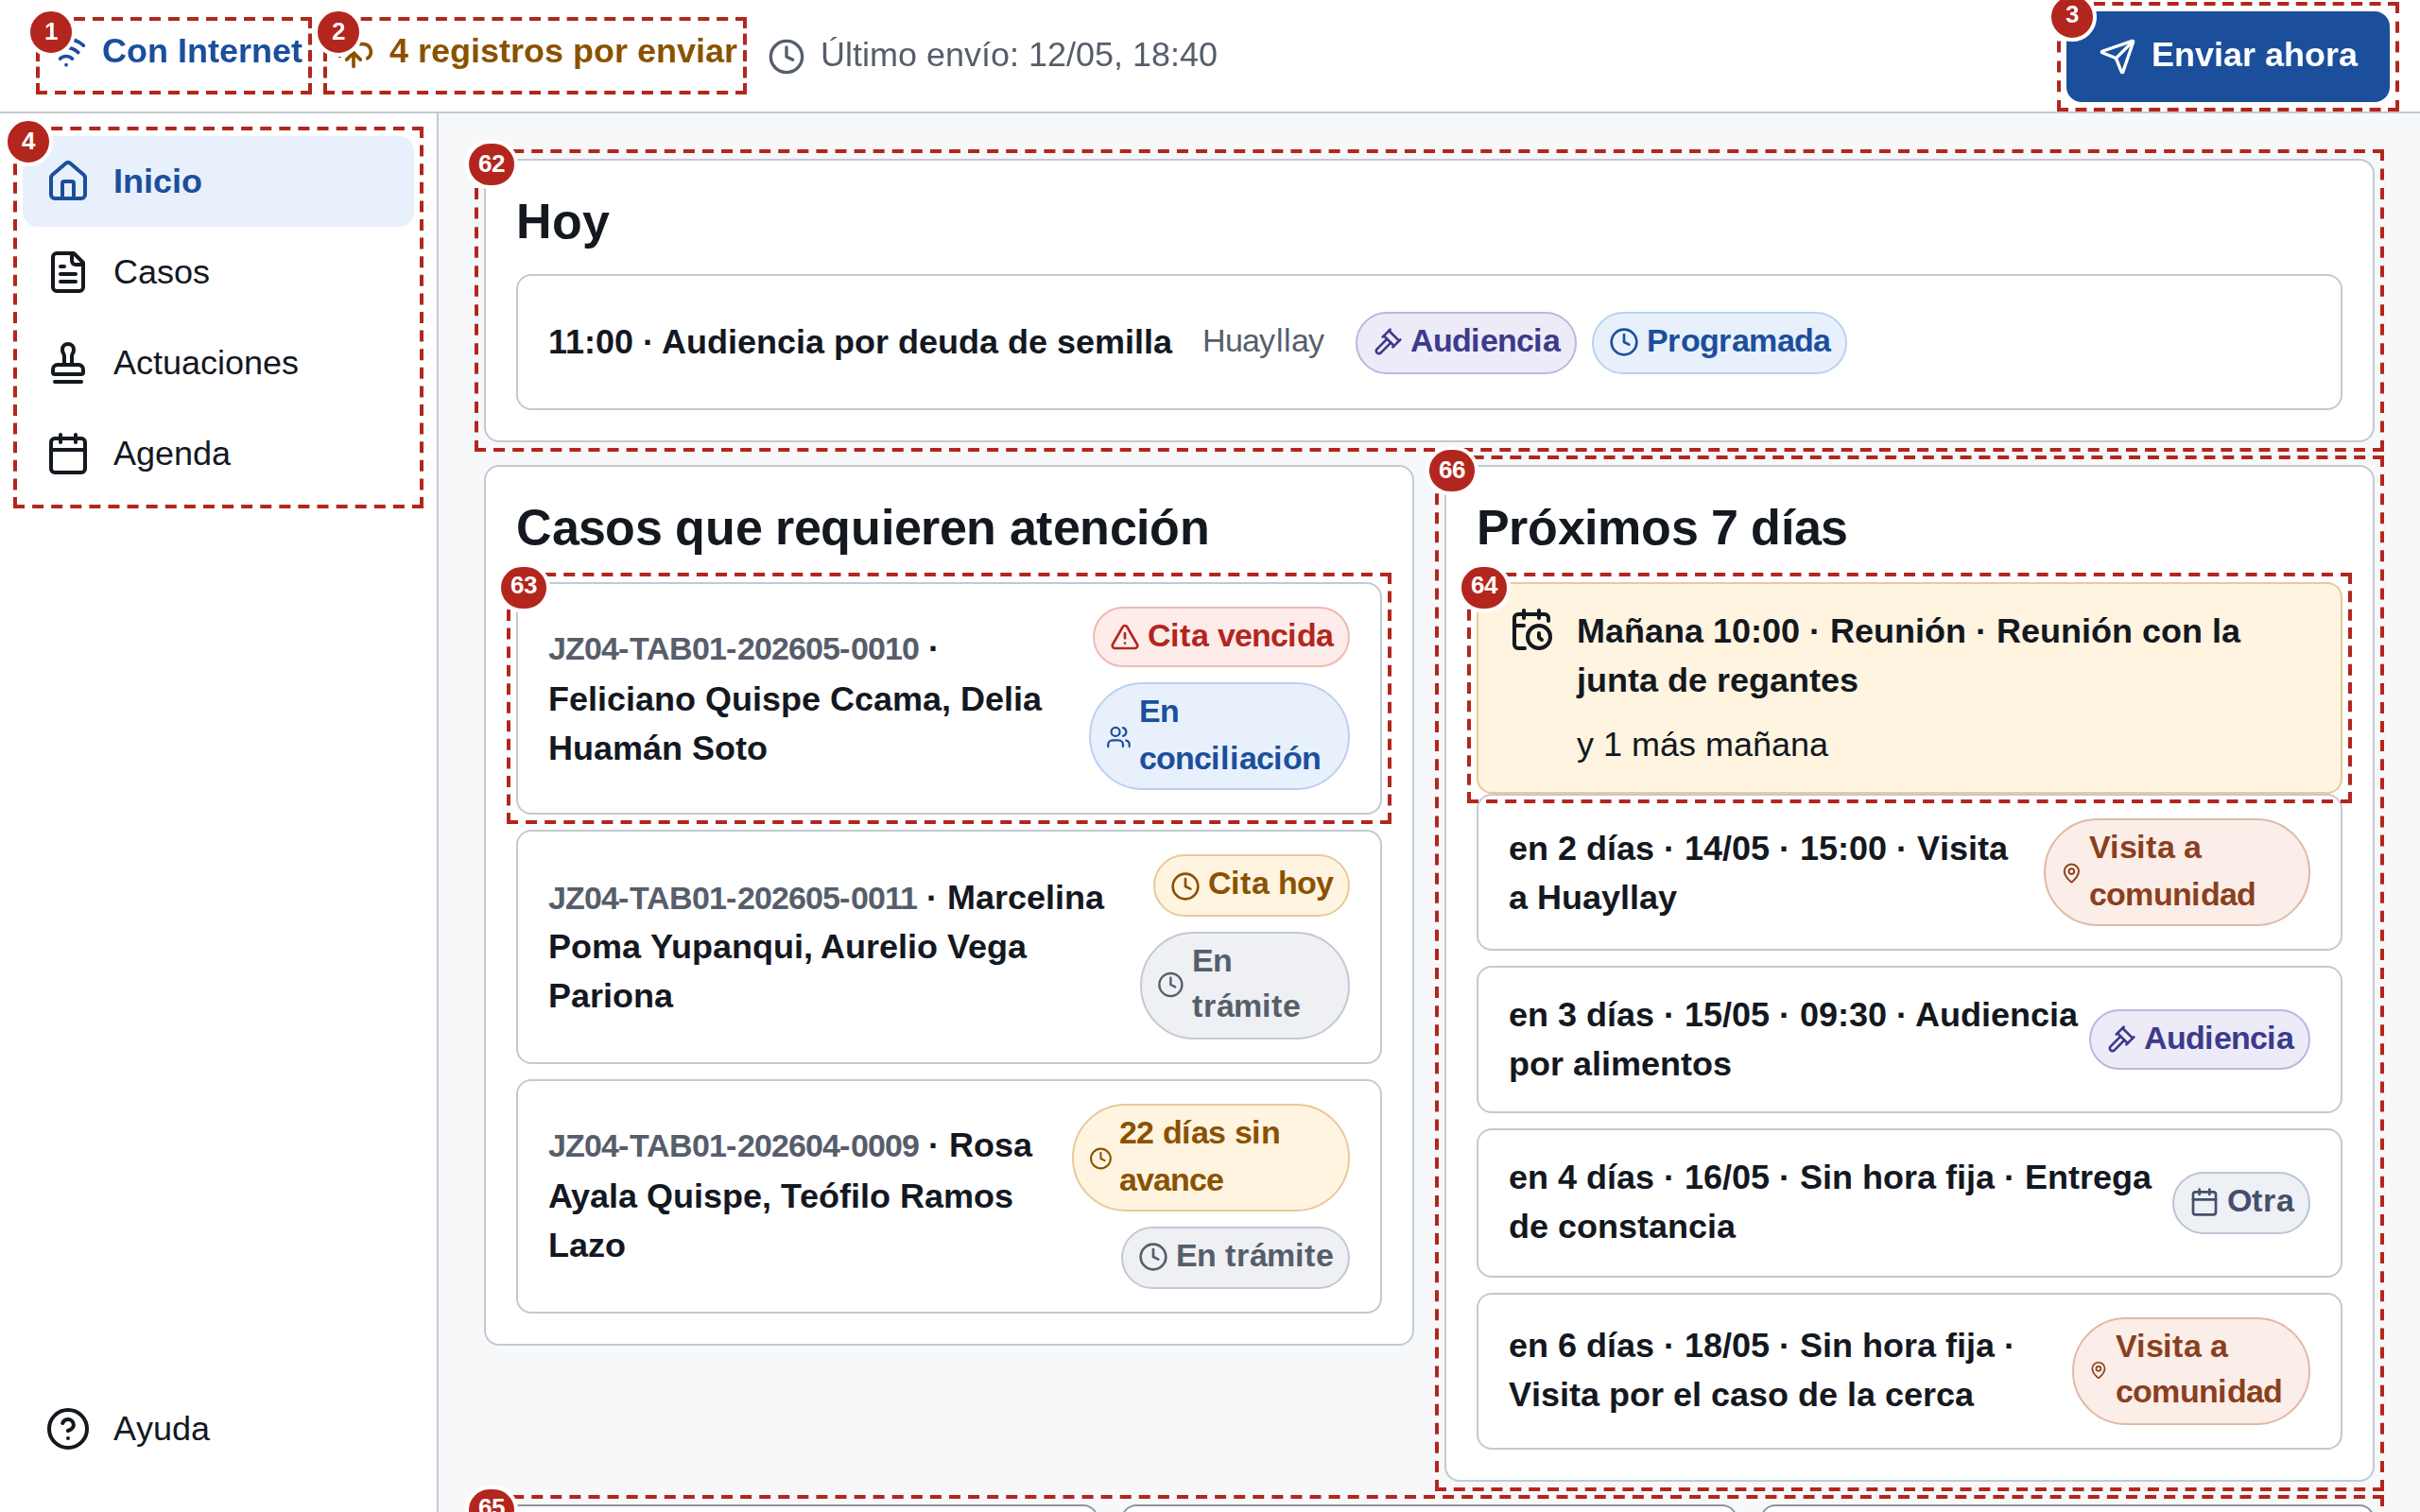
\includegraphics[width=0.86\linewidth]{capturas/A-01_anotada-inicio.png}
\caption{P-01 · Marcadores de la matriz. Cada marcador numerado corresponde a una fila de la matriz de justificación}
\end{figure}
\begin{figure}[H]\centering
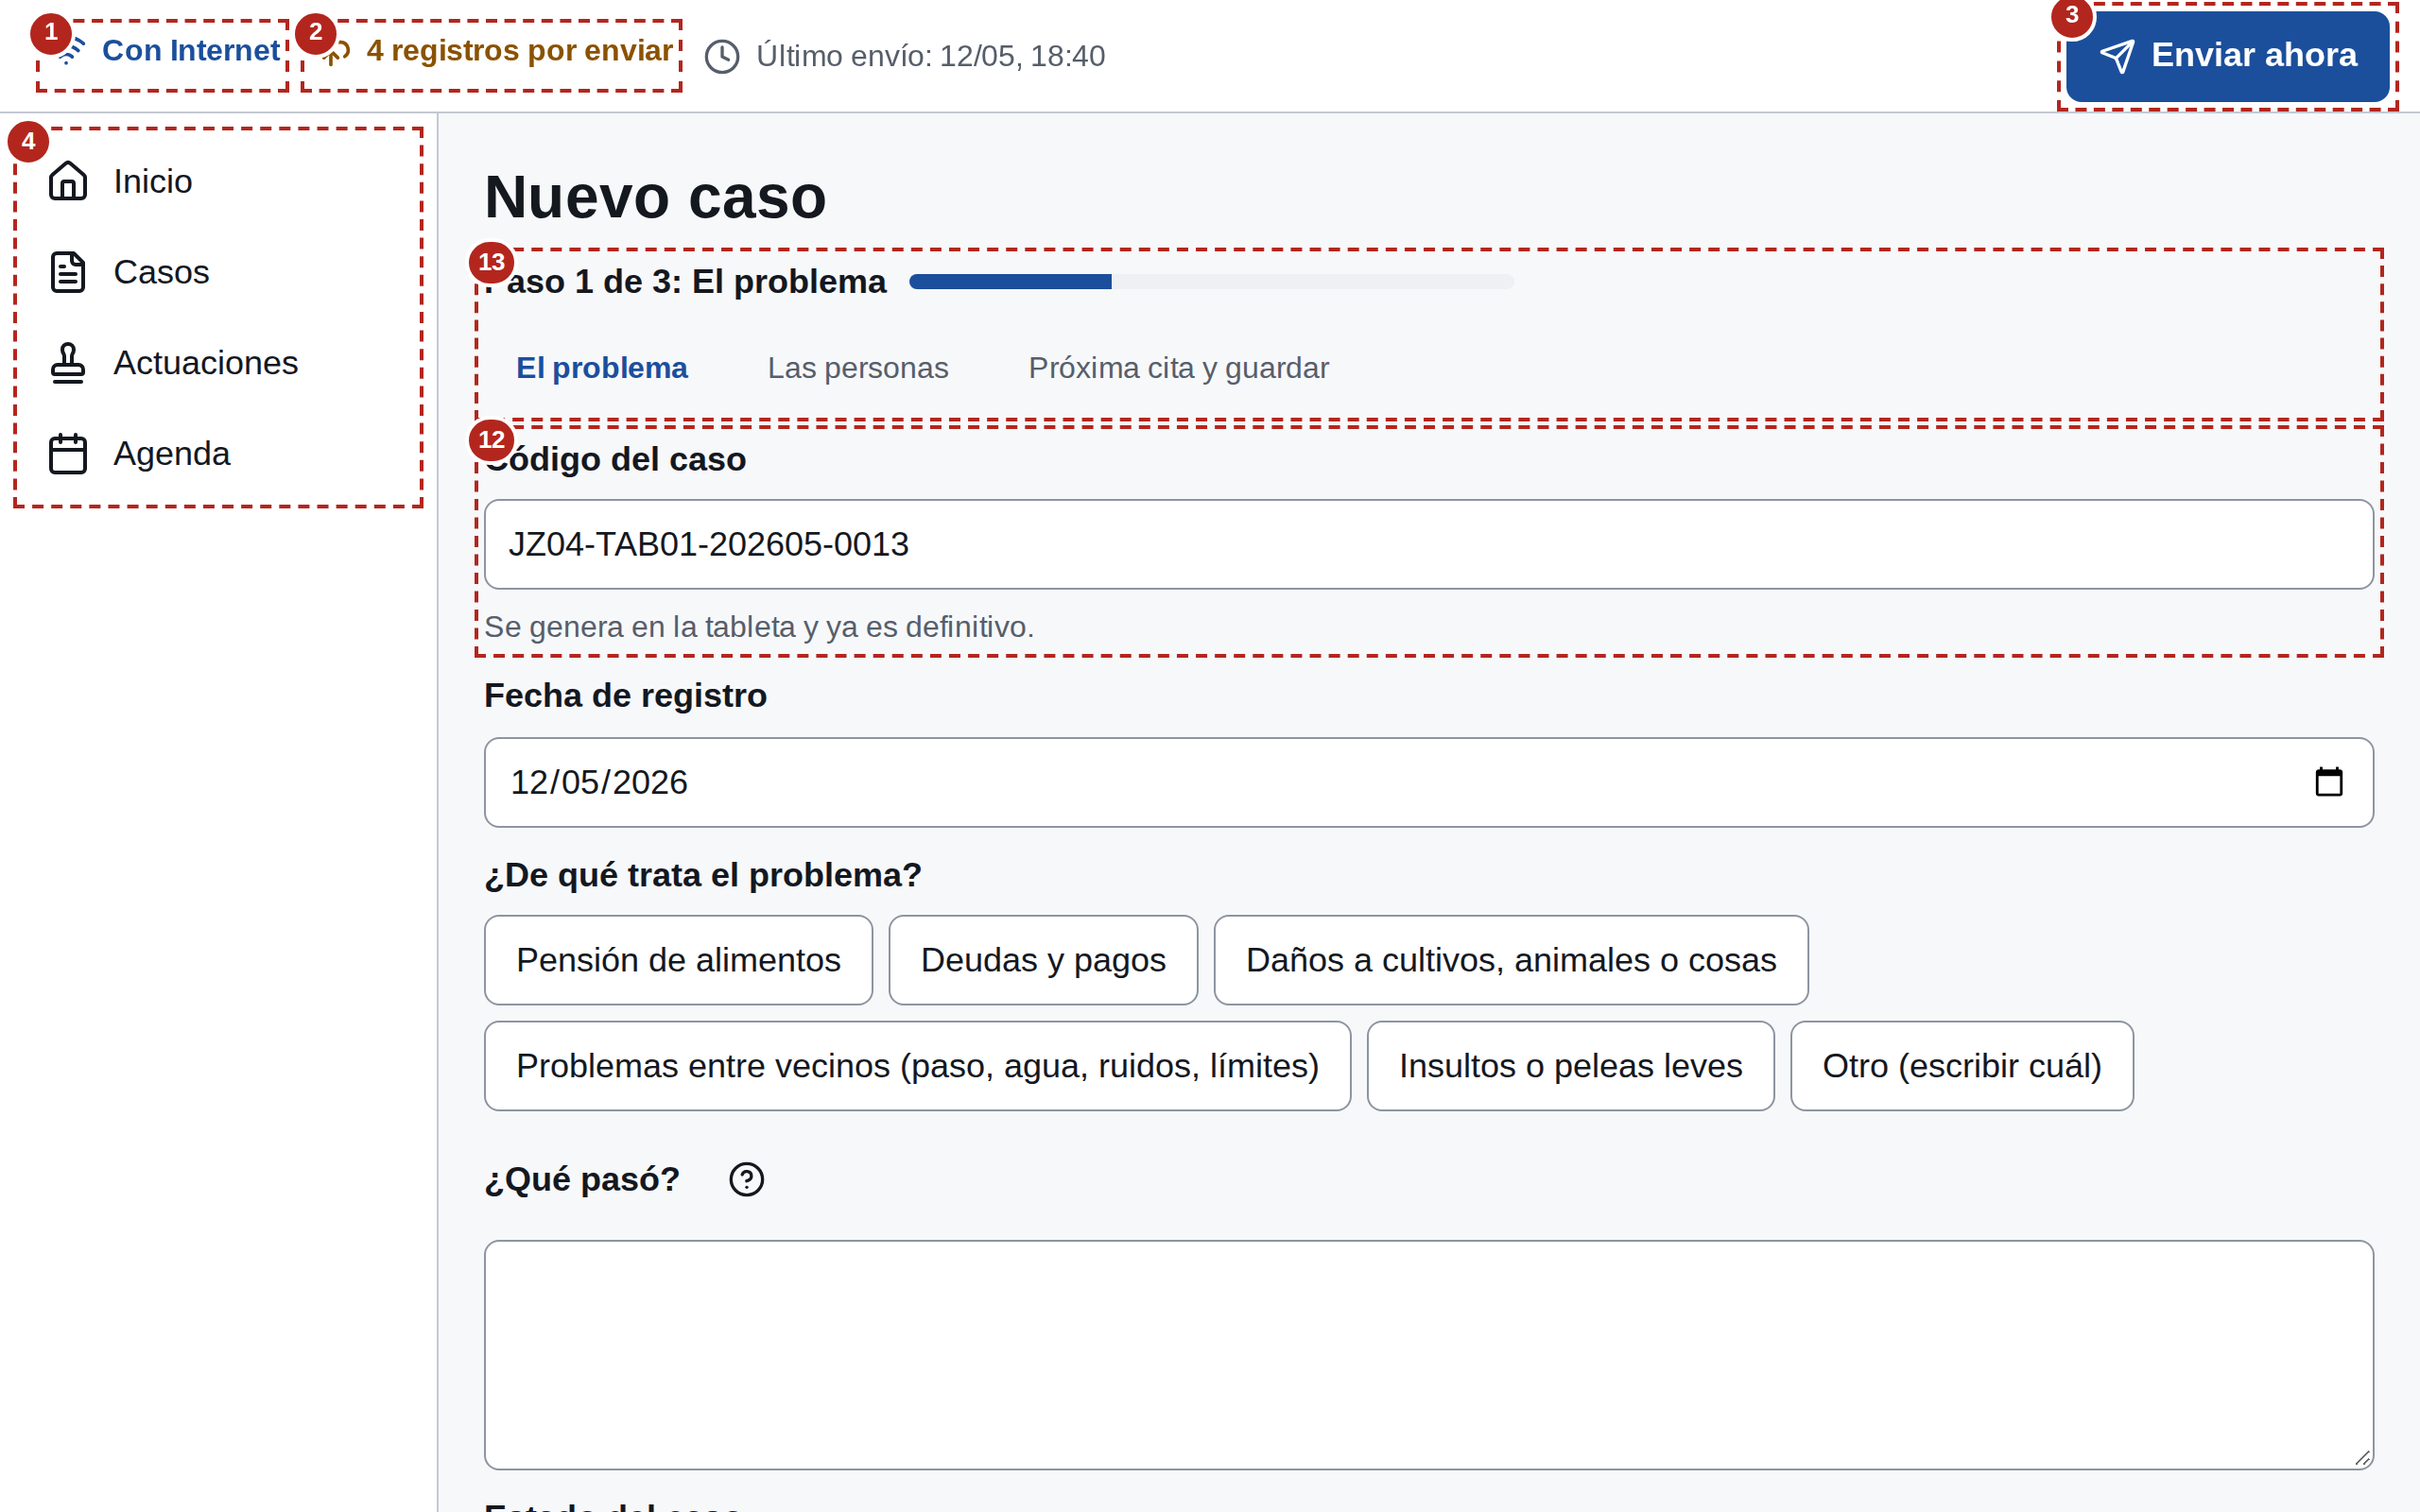
\includegraphics[width=0.86\linewidth]{capturas/A-02_anotada-caso.png}
\caption{P-03 · Marcadores de la matriz. Cada marcador numerado corresponde a una fila de la matriz de justificación}
\end{figure}
\begin{figure}[H]\centering
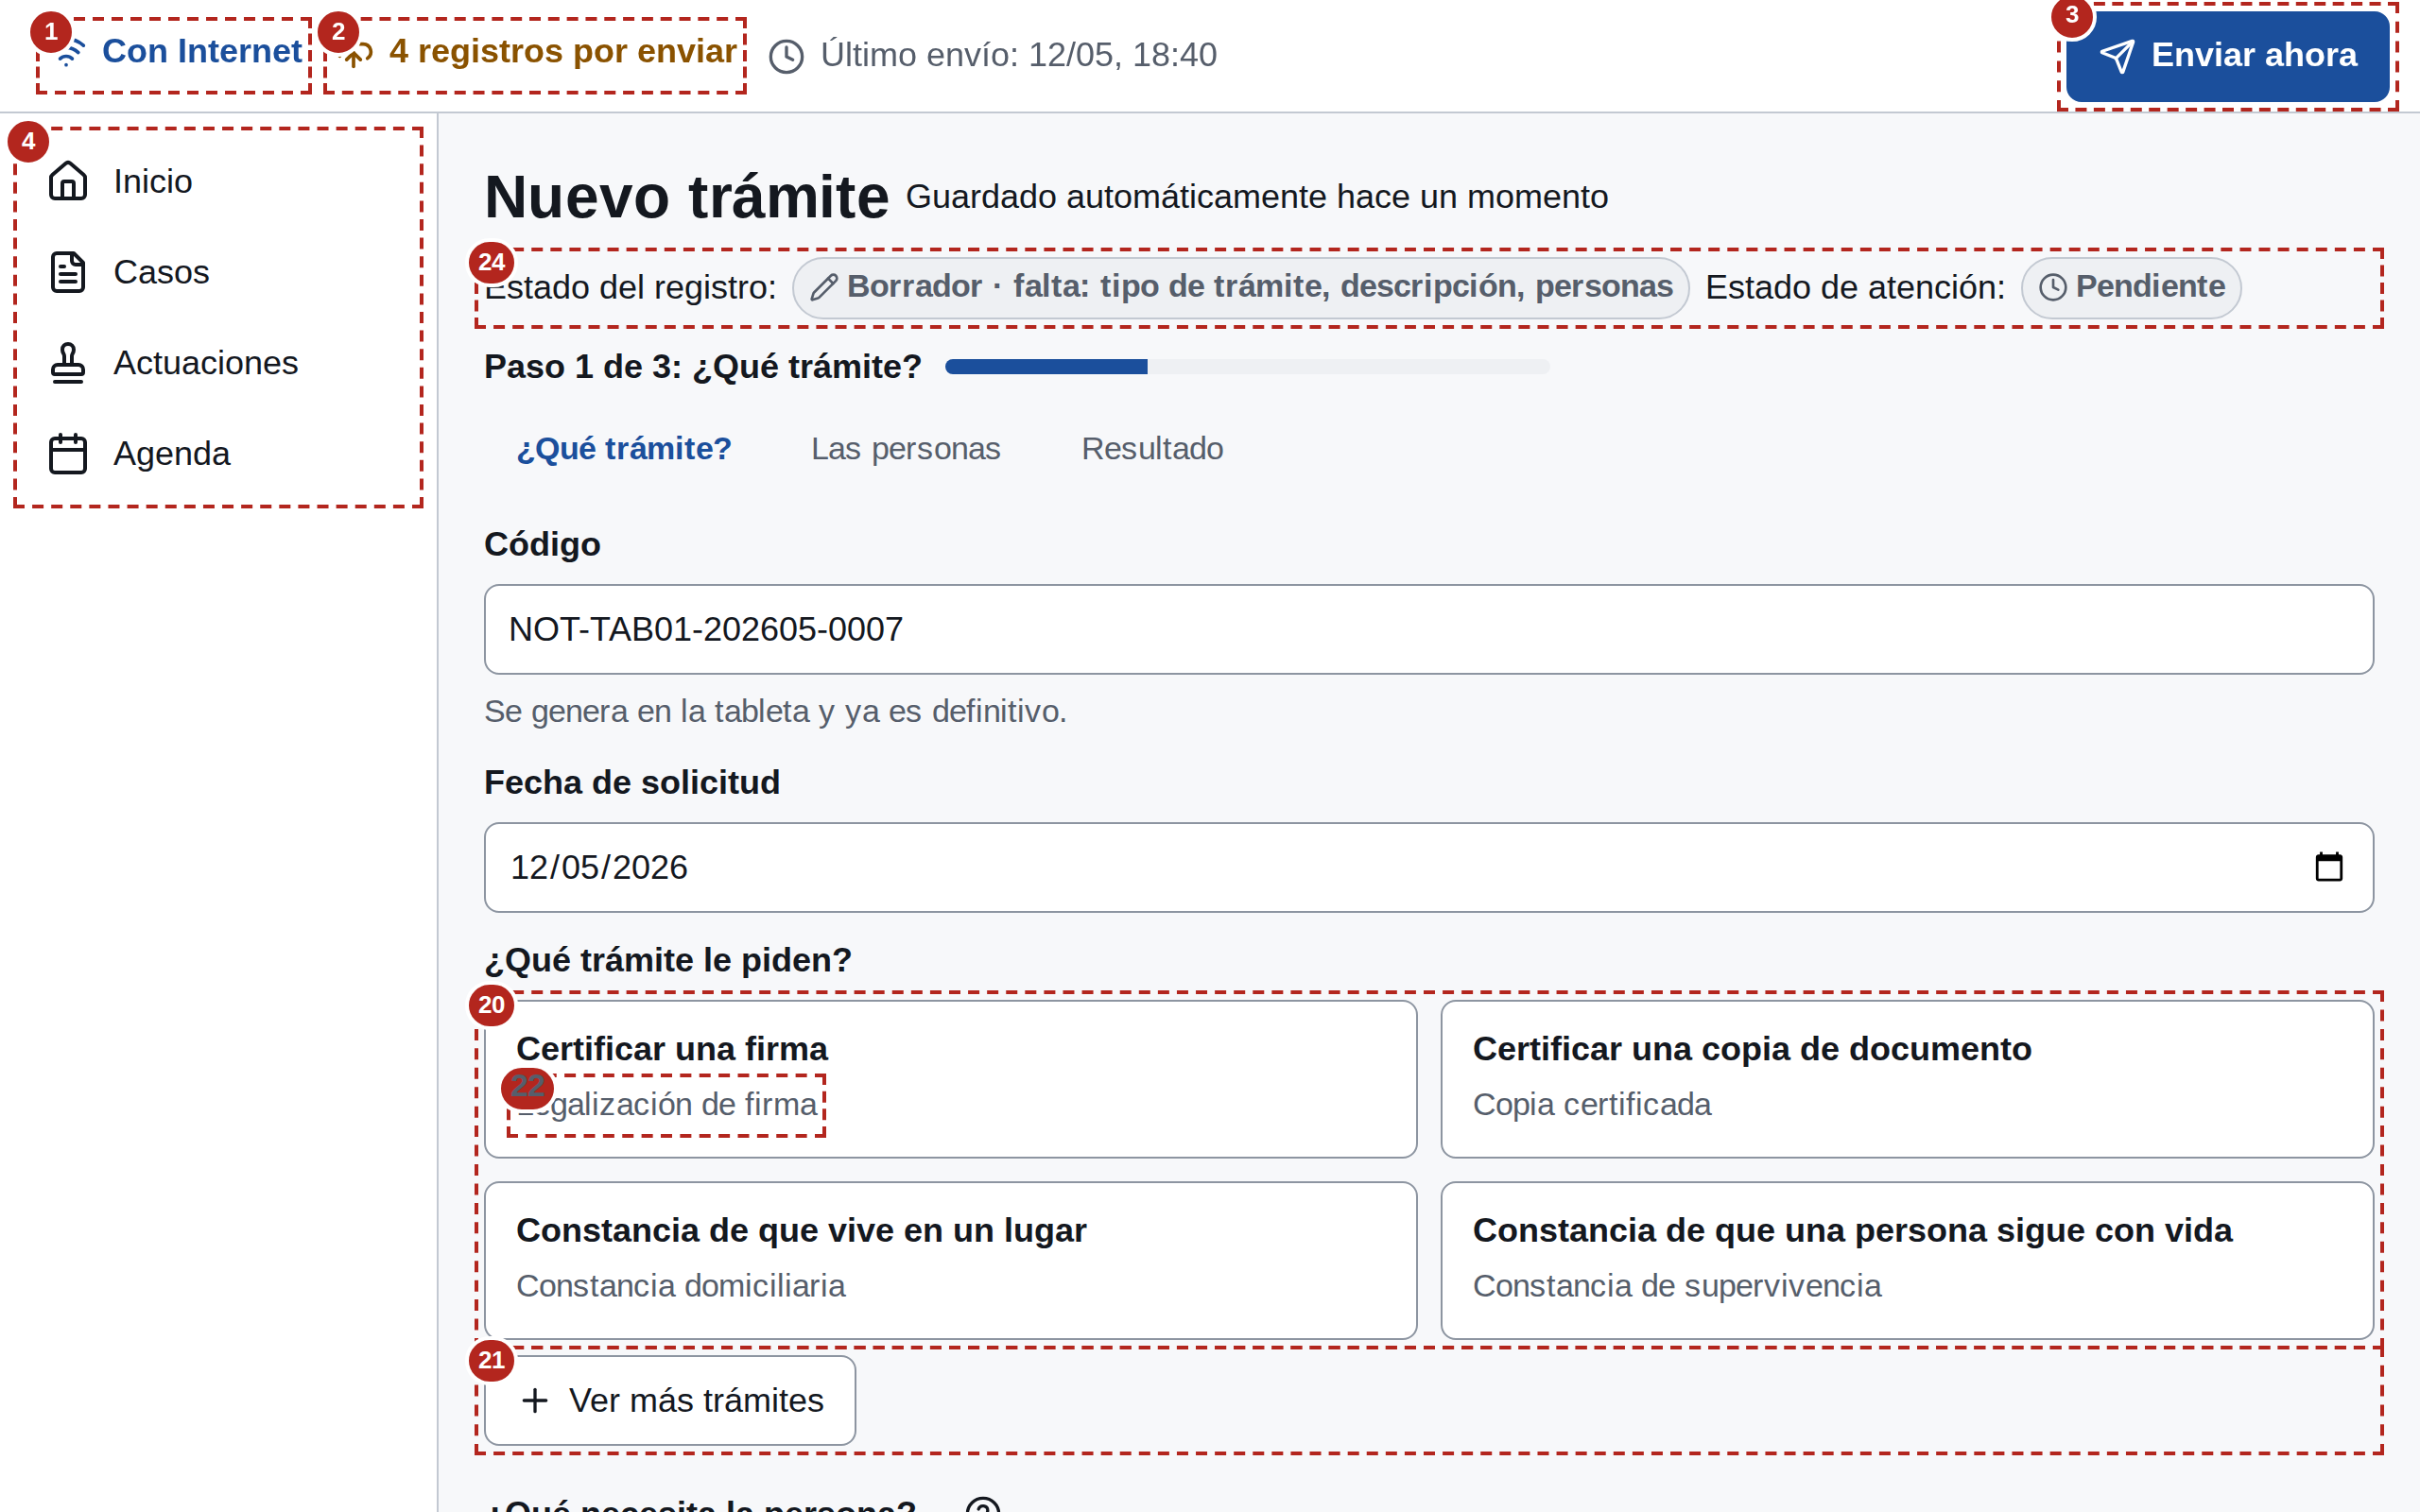
\includegraphics[width=0.86\linewidth]{capturas/A-03_anotada-actuacion.png}
\caption{P-06 · Marcadores de la matriz. Cada marcador numerado corresponde a una fila de la matriz de justificación}
\end{figure}
\begin{figure}[H]\centering
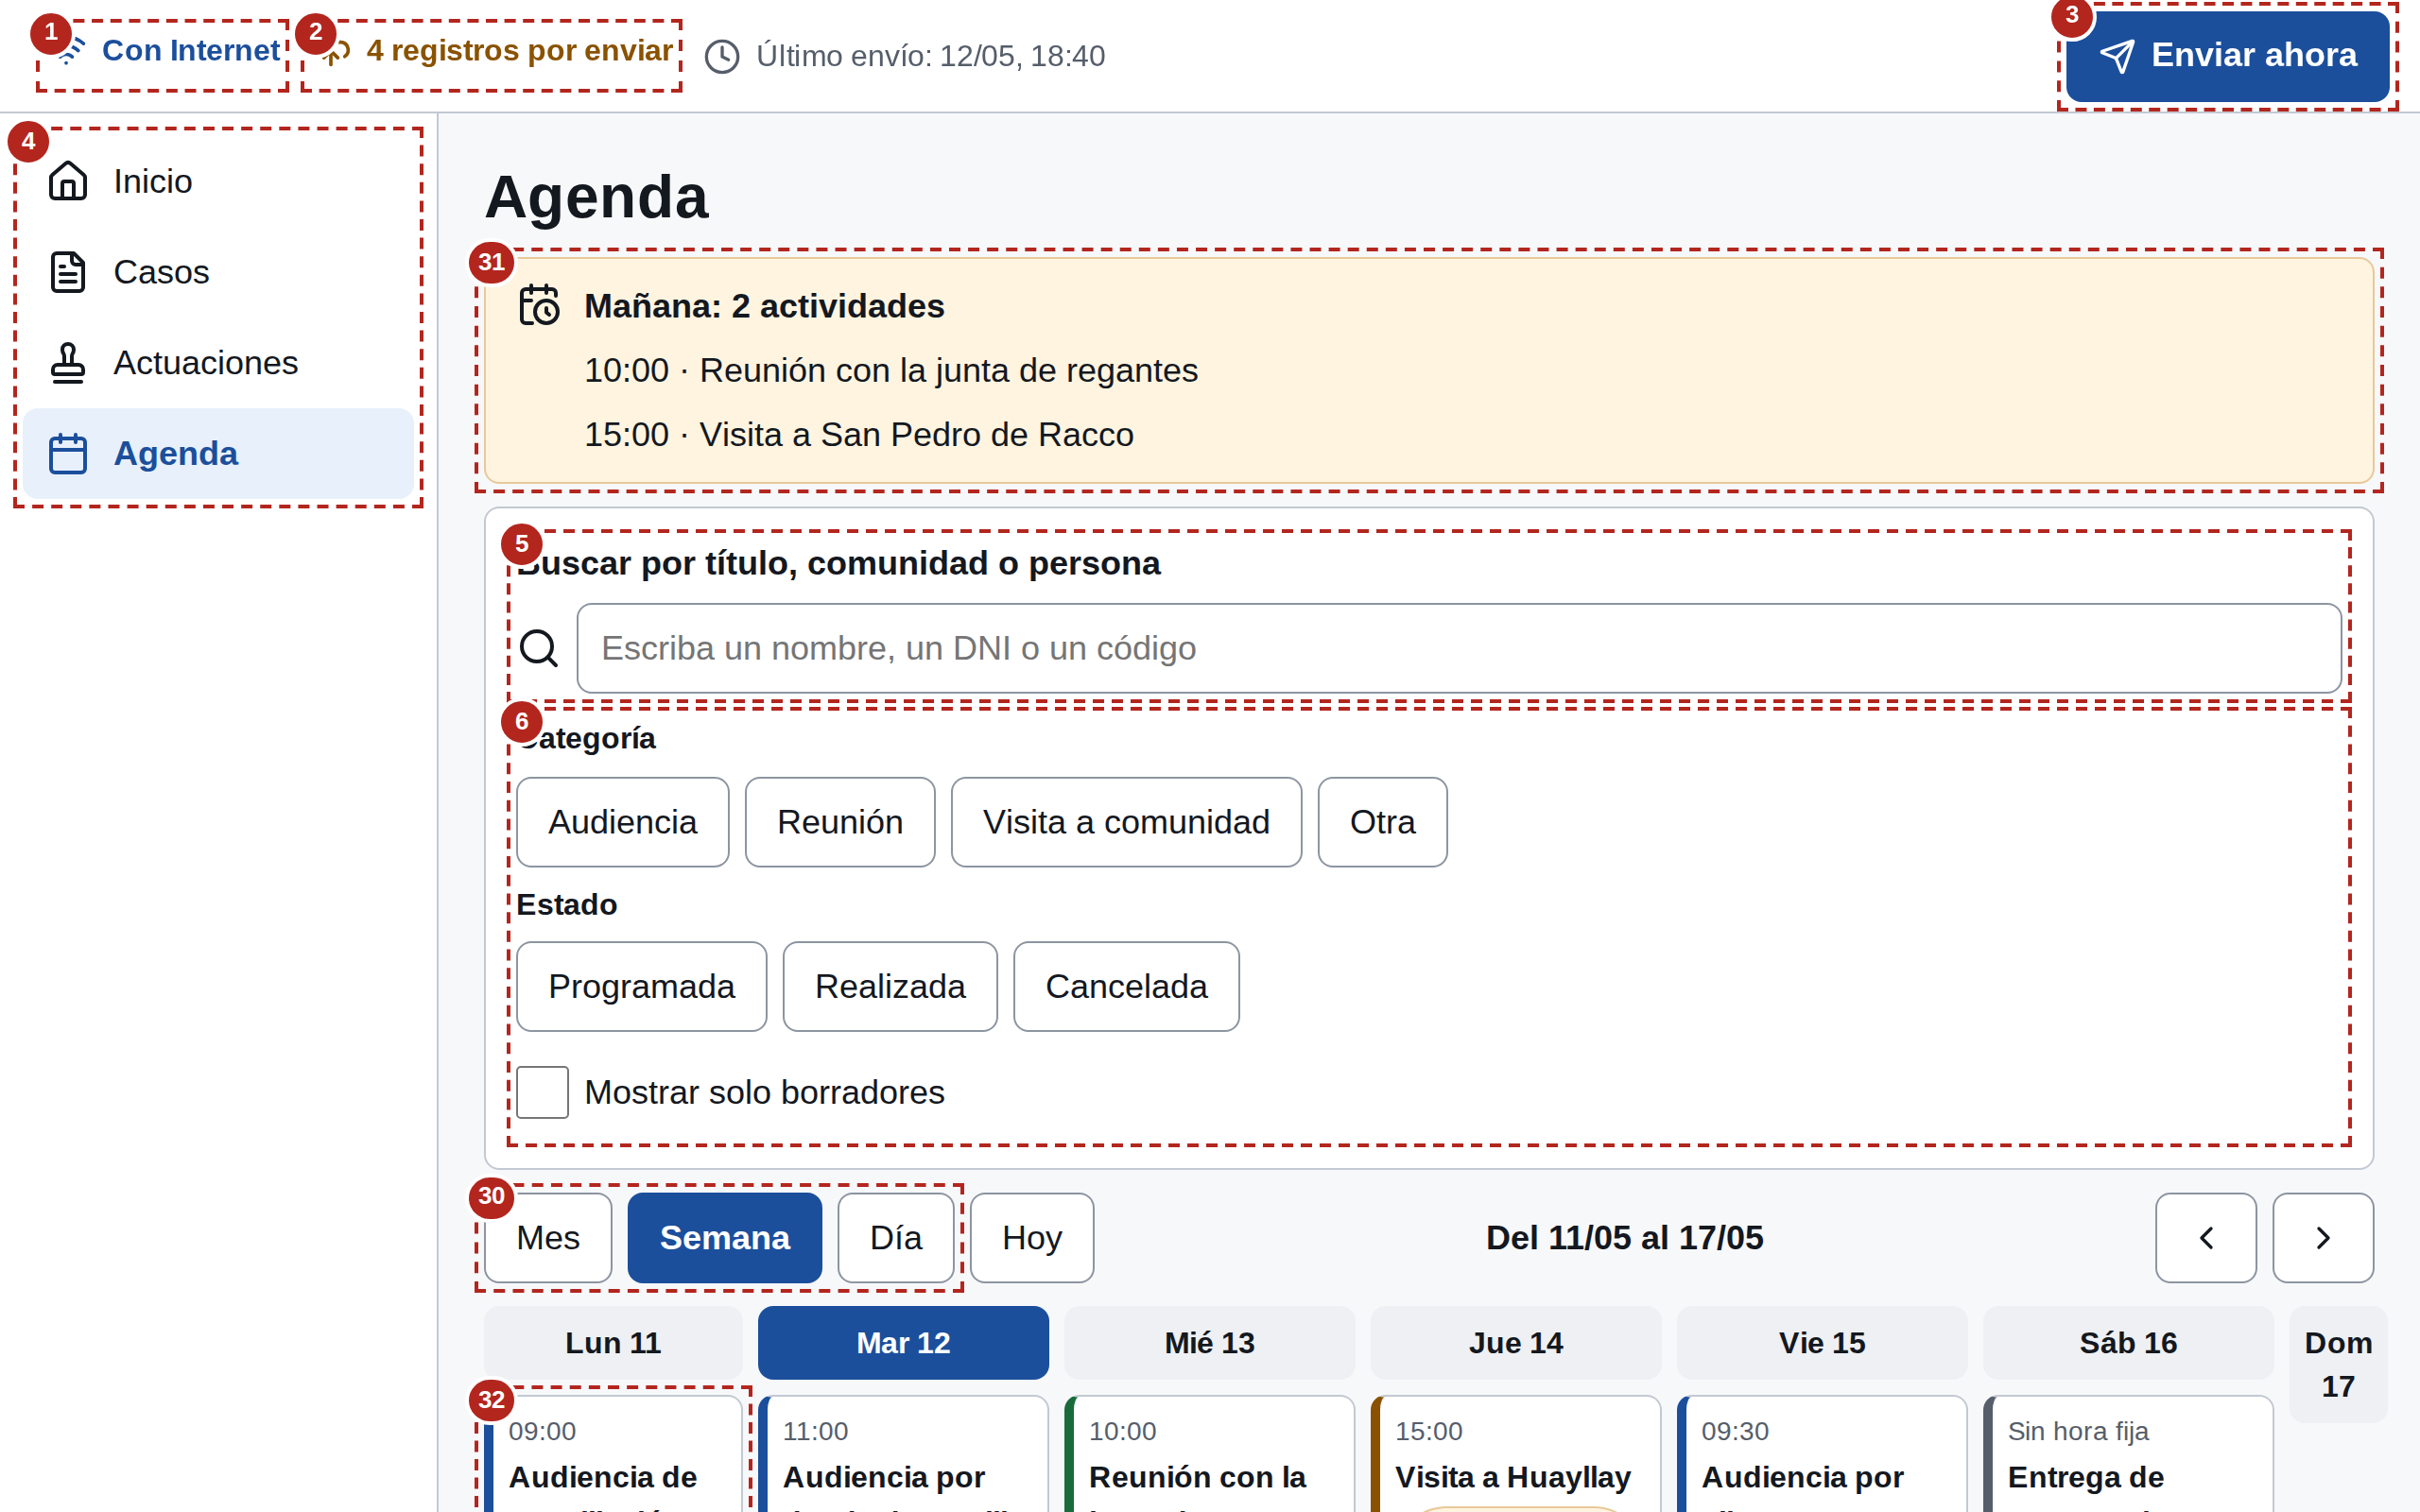
\includegraphics[width=0.86\linewidth]{capturas/A-04_anotada-agenda.png}
\caption{P-07 · Marcadores de la matriz. Cada marcador numerado corresponde a una fila de la matriz de justificación}
\end{figure}
\begin{figure}[H]\centering
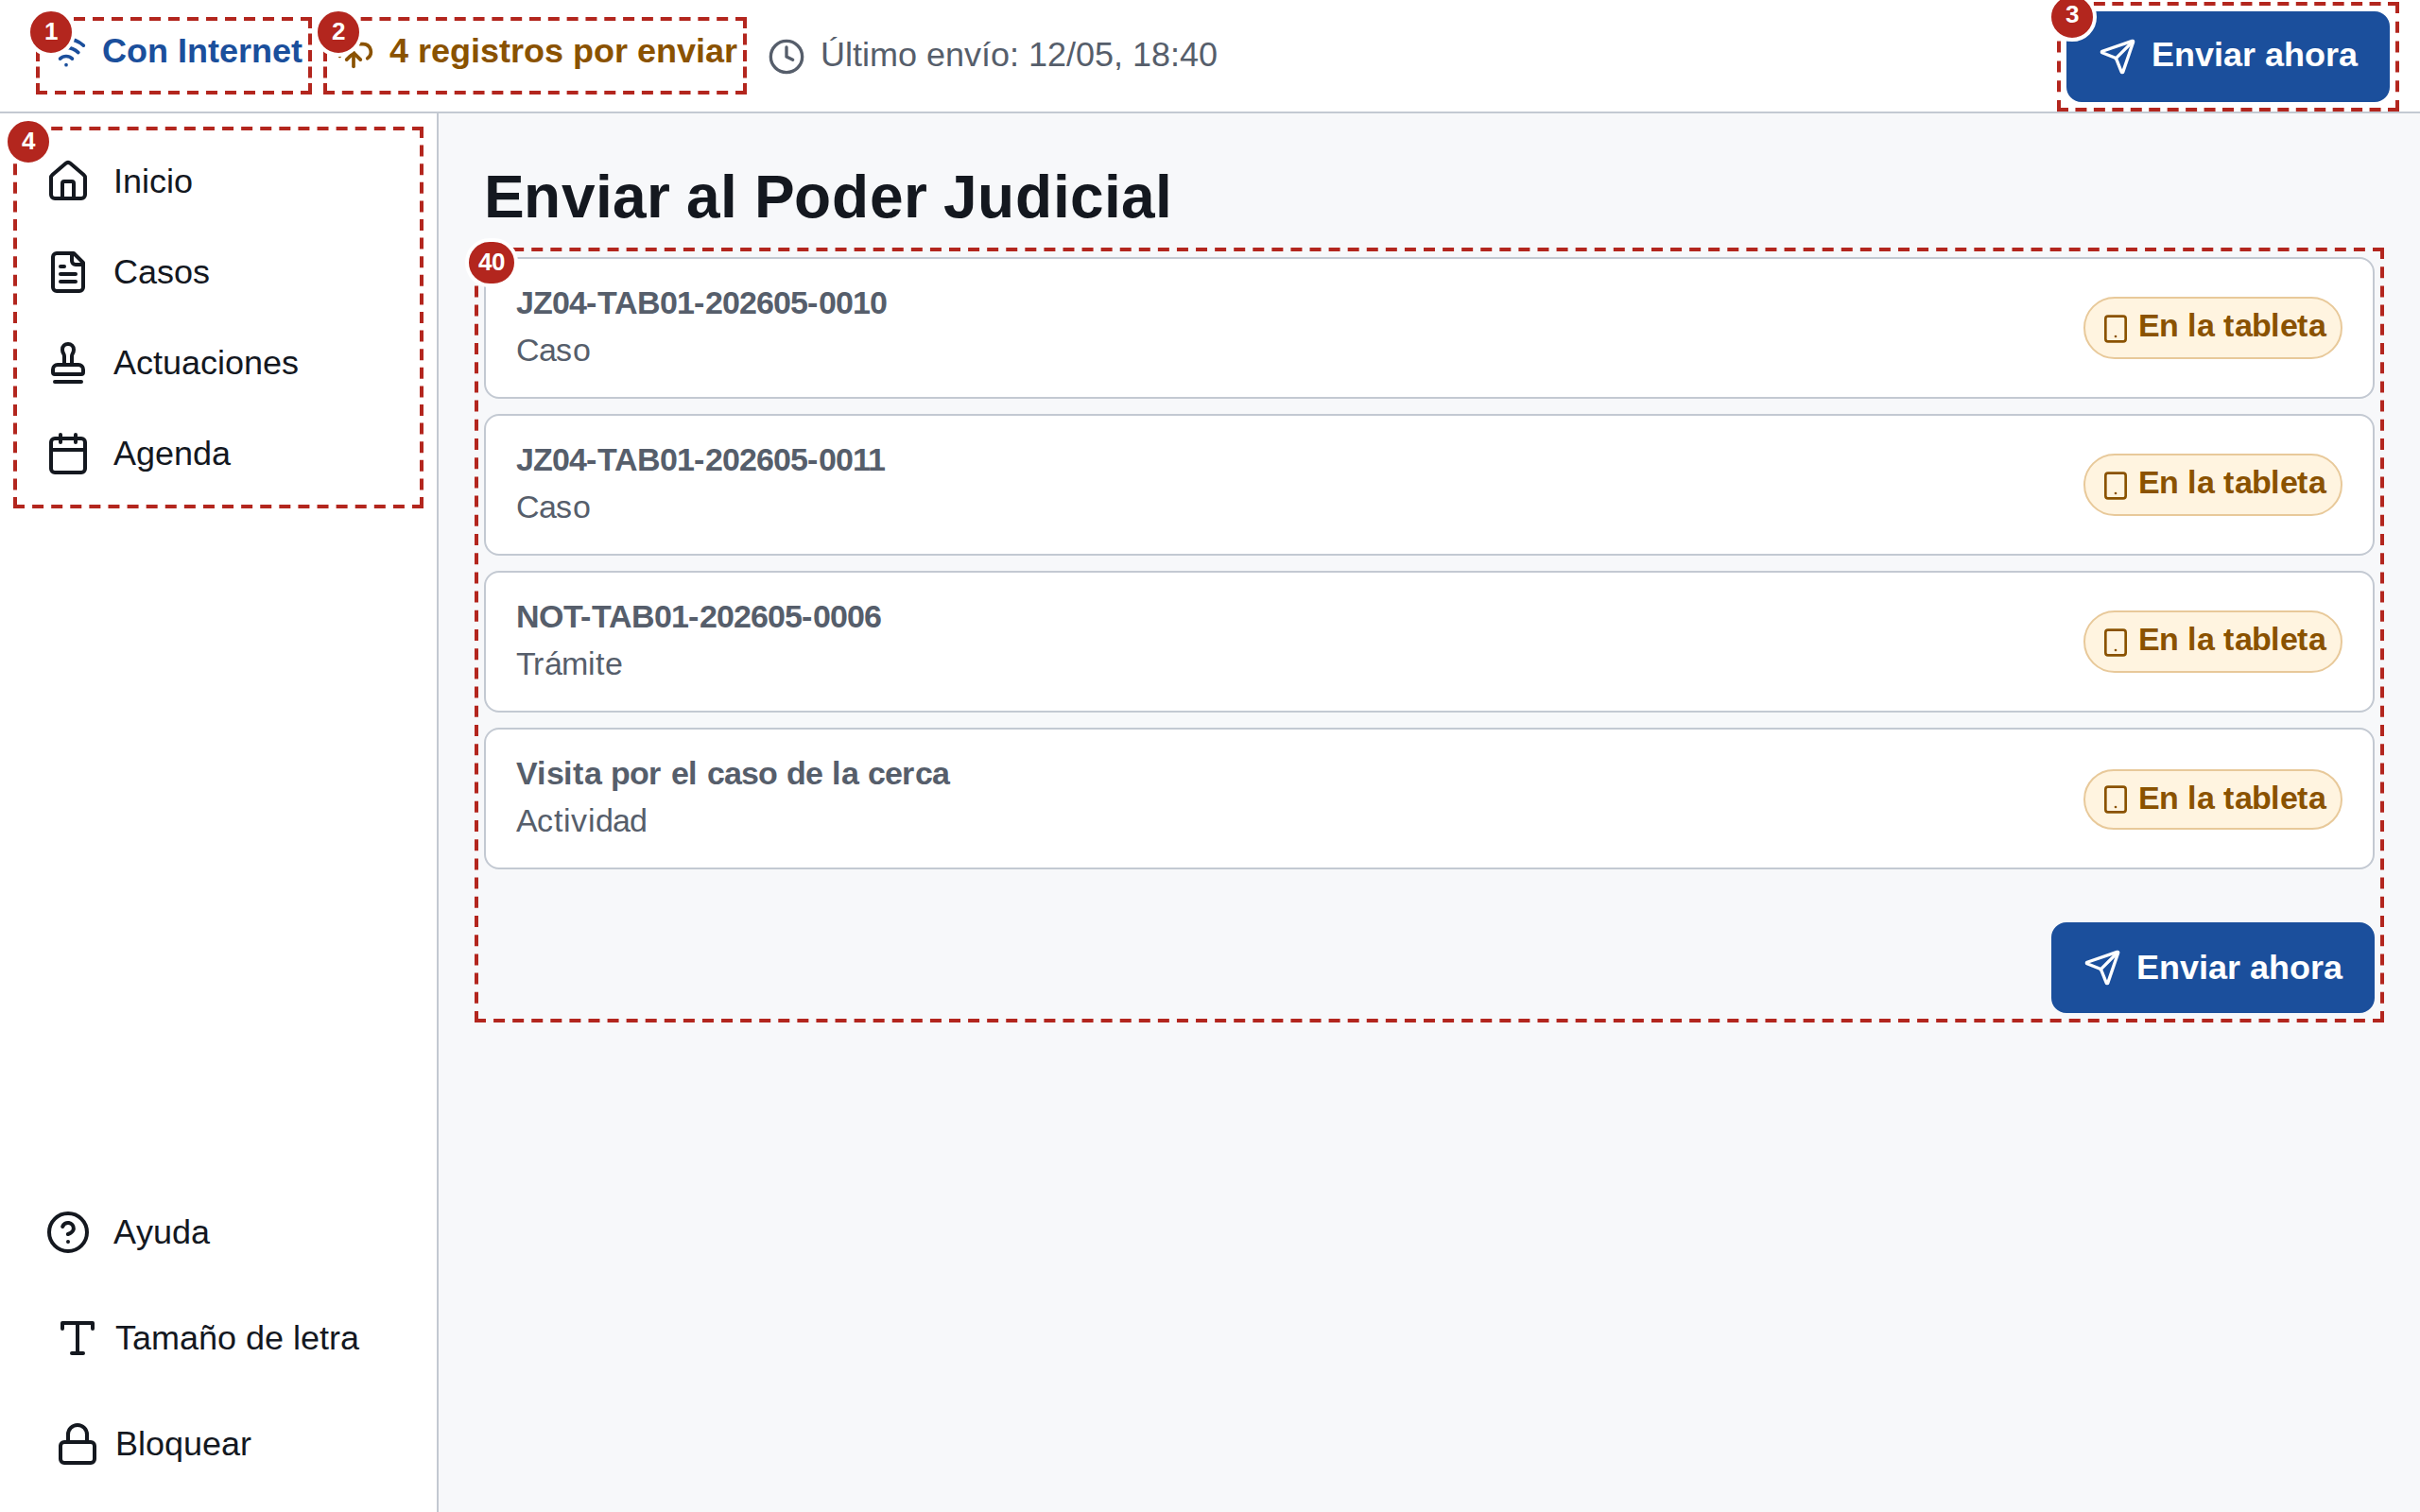
\includegraphics[width=0.86\linewidth]{capturas/A-05_anotada-envio.png}
\caption{P-09 · Marcadores de la matriz. Cada marcador numerado corresponde a una fila de la matriz de justificación}
\end{figure}
